%Template pembuatan proposal skripsi.
\documentclass{jtetiproposalskripsi}

%-----------------------------------------------------------------
%Disini awal masukan untuk data proposal skripsi
%-----------------------------------------------------------------
\titleind{IMPLEMENTASI SISTEM WIRELESS SECURITY DAN MANAJEMEN

BANDWIDTH BERBASIS RADIUS (REMOTE AUTHENTICATION DIAL

IN USER SERVICE) SERVER DENGAN MIKROTIK
}

\fullname{SHADIQUL HASAN SAIFURRIJAL}

\idnum{1110651225}

\approvaldate{20 Desember 2014}

\degree{Sarjana Komputer}

\yearsubmit{2014}

\program{Teknik Informatika}

\headprogram{Sarjiya, S.T., M.T., Ph.D.}

\dept{Teknik}

\firstsupervisor{Ari Eko Wardoyo, S.T., M.Kom}
\firstnip{1975 0214 2005 01 1 001}

\secondsupervisor{}
\secondnip{}


%-----------------------------------------------------------------
%Disini akhir masukan untuk data proposal skripsi
%-----------------------------------------------------------------

\begin{document}

\cover

\approvalpage

%-----------------------------------------------------------------
%Disini akhir masukan untuk muka skripsi
%-----------------------------------------------------------------

%-----------------------------------------------------------------
%Disini awal masukan Intisari
%-----------------------------------------------------------------
\begin{abstractind}
Salah satu perubahan utama di bidang telekomunikasi adalah penggunaan teknologi nirkabel (wireless). Masalah yang akan kita hadapi apabila menerapkan wireless LAN adalah isu tentang keamanannya. Banyak pihak yang masih mempertanyakan tentang keamanan wireless LAN.Apabila kita mengimplementasikan wireless LAN, maka kita juga harus mengimplementasikasistem keamanan apa yang akan kita terapkan. Solusi atau penanganan yang dilakukan adalah dengan menggunakan RADIUS (Remote Authentication Dial-In
User Service) server. RADIUS server memiliki protokol AAA (Authentication,Authorization, Accounting) yang dapat mengatur mekanisme bagaimana tata cara berkomunikasi, baik an ntara client ke domain-domain jaringan maupun antar client dengan domain yang berbeda dengan tetap menjaga keamanan pertukaran data.Metode pengembangan sistem yang penulis gunakan dalam penelitian ini adalah Security Policy Development Life Cycle (SPDLC). Dengan pengujian RADIUS server yang diimplementasikan pada jaringan hotspot Lembaga Ketahanan Nasional (LEMHANNAS) Republik Indonesia, diharapkan sistem RADIUS server ini dapat berjalan dengan baik serta cukup efisien dan praktis dalam
menangani permasalahan-permasalahan jaringan hotspot.





\bigskip
\textbf{Kata kunci} : \emph{RADIUS Server}, \emph{AAA}, \emph{SPLDC}
\end{abstractind}
%-----------------------------------------------------------------
%Disini akhir masukan Intisari
%-----------------------------------------------------------------

\tableofcontents
\addcontentsline{toc}{chapter}{DAFTAR ISI}
\selectlanguage{bahasa}\clearpage\pagenumbering{arabic}\setcounter{page}{1}

%-----------------------------------------------------------------
%Disini awal masukan untuk Bab
%-----------------------------------------------------------------
\chapter{LATAR BELAKANG}

\section{Latar Belakang Masalah}
Salah satu perubahan utama di bidang telekomunikasi adalah penggunaan teknologi nirkabel (wireless). Teknologi wireless juga diterapkan padajaringan komputer, yang lebih dikenal dengan wireless LAN (WLAN).Kemudahan-kemudahan yang ditawarkan wireless LAN menjadi daya tarik tersendiri bagi para pengguna komputer dalam menggunakan teknologi ini untuk mengakses suatu jaringan komputer atau internet.


Masalah yang akan kita hadapi apabila menerapkan wireless LAN adalah isu tentang keamanannya. Banyak pihak yang masih mempertanyakan tentang keamanan wireless LAN. Apabila kita mengimplementasikan wireless LAN,maka kita juga harus mengimplementasikan sistem keamanan apa yang akan kita terapkan. Banyak hotspot yang tidak menerapkan sistem keamanan yang
memadai, sehingga memungkinkan pengguna yang tidak berhak (ilegal) dapat masuk ke jaringan hotspot tersebut. Apabila hal ini sampai terjadi, maka pemilik hotspot tersebut secara langsung maupun tidak langsung akan dirugikan, penyusup itu dapat saja melakukan perbuatan yang tidak menyenangkan, seperti mengambil data, dan menyerang komputer-komputer yang ada di jaringan tersebut.


Sistem keamanan yang paling umum diterapkan pada wireless LAN adalah dengan metode enkripsi, yaitu WEP (Wired Equivalent Privacy). WEP ini menggunakan satu kunci enkripsi yang digunakan bersama-sama oleh para pengguna wireless LAN. Hal ini menyebabkan WEP tidak dapat diterapkan pada hotspot yang dipasang di tempat-tempat umum. Dan karena lubang keamanan yang dimiliki WEP cukup banyak, sehingga mudah dibobol oleh pihak ketiga yang tidak berhak, maka penggunaannya tidak disarankan lagi.

Sistem keamanan lainnya adalah WPA (Wi-Fi Protected Access), yang menggeser WEP dan menghasilkan keamanan yang lebih baik dari WEP.WPA bersifat meminta network key kepada setiap wireless client yang ingin melakukan koneksi ke jaringan. Kekurangan dari WPA ini adalah kurang optimal dalam pelayanan, dikarenakan setiap user yang ingin mengakses jaringan diharuskan membawa perangkat wireless-nya untuk meminta network key kepada administrator (tidak praktis). Serta tidak adanya sistem informasi bandwidth,user management,dan monitoring membuat administrator tidak dapat memantau serta mengontrol user maupun melakukan manajemen bandwidth di dalam jaringan wireless LAN (hotspot).

Saat ini, sistem kemanan jaringan wireless LAN yang ada di lingkungan Lembaga Ketahanan Nasional (LEMHANNAS) sangatlah minim, bahkan bisa dibilang tidak menggunakan sistem keamanan yang memadai, karena tidak adanya sistem autentikasi untuk pengguna hotspot. Oleh karena itu saya sebagai penulis dan peneliti tertarik untuk menerapkan sebuah sistem keamanan
jaringan wireless yang berbasiskan RADIUS(Remote Authentication Dial In User Service). Sistem RADIUS server ini diharapkan dapat membantu administrator jaringan untuk dapat memantau serta 
mengontrol user dan melakukan manajemen bandwidth di dalam jaringan wireless LAN (hotspot) yang ada di LEMHANNAS. User yang dimaksud adalah pengguna jaringan wireless, yatiu pegawai dan tamu yang ada di lingkungan LEMHANNAS.



\section{Tujuan Penelitian}
Penelitian ini bertujuan untuk mengidentifikasi kebutuhan sistem
jaringan nirkabel dan memberikan solusi pada permasalahan dalam
menangani AAA (Authentication, Authorization, Accounting). Yang pada intinya adalah menangani otentikasi user, otorisasi untuk servis-servis, dan penghitungan nilai servis yang digunakan user. Selain itu juga, untuk mengetahui sistem keamanan jaringan wireless serperti apa yang tepat diterapkan di LEMHANNAS.


\section{Manfaat Penelitian}

1. Dapat memudahkan dalam memberikan hak akses pada pengguna
   layanan, serta mengklasifikasikan para pengguna tersebut.

2. Dapat memudahkan dalam mengontrol para pengguna jaringan
   nirkabel.

3. Dapat memudahakan dalam memantau para pengguna jaringan
   nirkabel (data record).



%-------------------------------------------------------------------------------
\chapter{DASAR TEORI}                

\section{Landasan Teori}
\subsection{Jaringan (Network)}


	Jaringan (network) adalah kumpulan dua atau lebih komputer yang
masing-masing berdiri sendiri dan terhubung melalui sebuah teknologi.Hubungan antar komputer tersebut tidak terbatas berupa kabel tembaga saja,namun juga bisa melalui fiber optic, microwave, infrared , bahkan melalui satelit (Tanenbaum, 2003, p10).

Tujuan dari penggunaan jaringan komputer adalah :

1. Membagi sumber daya : contohnya berbagi pemakain printer,CPU,
   memori, dan harddisk.

2. Komunikasi : contohnya surat elektronik, instant messaging,             dan chatting.

3. Akses informasi : contohnya web browsing. 

Secara umum jaringan mempunyai beberapa manfaat yang lebih
dibandingkan dengan komputer yang berdiri sendiri. Adapun manfaat yang didapat dalam membangun suatau jaringan adalah sebagai berikut :

1. Sharing resources.

2. Media komunikasi.

3. Integrasi data.

4. Pengembangan dan pemeliharaan.

5. Keamanan data.

6. Sumber daya lebih efisien dan informasi terkini.


\subsection{Klasifikasi Jaringan Komputer}

A. Klasifikasi Jaringan Berdasarkan Tipe Transmisinya 				Berdasarkan tipe transmisinya (Tanebaum, 2003, p15), jaringan dibagi menjadi dua bagian besar yaitu : broadcast dan point to point.Dalam broadcoast network, komunikasi terjadi dalam sebuah saluran komunikasi yang digunakan secara bersama-sama, dimana data berupa paket yang dikirimkan dari sebuah komputer akan disampaikan ke tiap komputer yang ada dalam jaringan tersebut. Paket data hanya akan di proses oleh komputer tujuan dan akan dibuang oleh komputer yang bukan tujuan paket tersebut. Sedangkan pada point to point network, komunikasi data terjadi
melalui beberapa koneksi antar sepasang komputer, sehingga untuk
mencapai tujuannya sebuah paket mungkin harus melalui beberapa
komputer terlebih dahulu.
Oleh karena itu, dalam tipe jaringan ini,pemilihan rute yang baik menentukan baik tidaknya koneksi data yang berlangsung.
\subsection{Klasifikasi Jaringan Berdasarkan Skalanya}
1. PAN (Personal Area Network)

\begin{figure}[ht!]
  \centering
    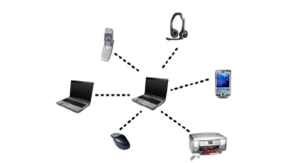
\includegraphics{gambar/pan}
    \caption{PAN (Personal Area Network)}
    \label{kripto}
\end{figure}
	PAN (Personal Area Network) adalah jaringan komputer yang digunakan untuk komunikasi antara peralatan komputer dengan user.Jangkauan dari PAN biasanya hanya beberapa meter saja (6-9 meter).PAN dapat digunakan untuk komunikasi antara perangkat pribadi sendiri (komunikasi intrapersonal), seperti pada PC dengan keyboard ataupun mouse. Beberapa contoh alat yang digunakan dalam PAN adalah printer, mesin fax, telephone, PDA atau scanner. PAN dapat dihubungkan dengan kabel dengan computer buses seperti USB dan firewire.

2. LAN (Local Area Network)

\begin{figure}[ht!]
  \centering
    \includegraphics{gambar/lan}
    \caption{LAN (Local Area Network)}
    \label{kripto}
\end{figure}

	LAN (Local Area Network) adalah sebuah jaringan komputer
yang dibatasi oleh area geografis yang relatif kecil dan umumnya
dibatasi oleh area lingkungan seperti perkantoran atau sekolahan dan biasanya ruang lingkup yang dicakupnya tidak lebih dari 2 km
(Stallings, 2000, p425).
Ciri-ciri LAN adalah sebagai berikut :

a. Beroperasi pada area yang terbatas.

b. Memiliki kecepatan transfer yang tinggi.

c. Dikendalikan secara privat oleh administrator lokal.

d. Menghubungkan peralatan yang berdekatan.

3. MAN (Metropolitan Area Network)

\begin{figure}[ht!]
  \centering
    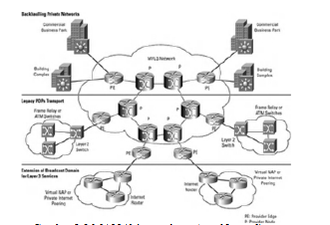
\includegraphics{gambar/man}
    \caption{MAN (Metropolitan Area Network)}
    \label{kripto}
\end{figure}
	
	MAN (Metropolitan Area Network) adalah suatu jaringan dalam suatu kota dengan transfer data berkecepatan tinggi,yang
menghubungkan berbagai lokasi seperti kampus, perkantoran, pemerintahan, dan sebagainya. Jaringan MAN adalah gabungan dari 
beberapa LAN. Jangkauan dari MAN adalah 10-50 km, MAN merupakan jaringan yang tepat untuk membangun suatu jaringan antar kantor-kantor dalam satu kota antara pabrik/instansi dan kantor pusat yang berada dalam jangkauannya.

4. WAN (Wide Area Network)
	
\begin{figure}[ht!]
  \centering
    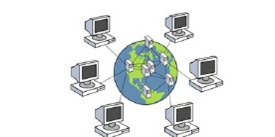
\includegraphics{gambar/wan}
    \caption{WAN (Wide Area Network)}
    \label{kripto}
\end{figure}
	
	WAN (Wide Area Network) merupakan jaringan yang ruang lingkupnya sudah terpisahkan oleh batas geografis dan biasanya sebagai penghubungnya sudah menggunakan media satelit ataupun kabel bawah laut (Stallings, 2000, p9).

Ciri-ciri WAN adalah sebagai berikut :

a. Beroperasi pada wilayah geografis yang sangat luas.

b. Memiliki kecepatan transfer yang lebih rendah daripada LAN.

c. Menghubungkan peralatan yang dipisahkan oleh wilayah yang
   luas, bahkan secara global.


\subsection{Klasifikasi Jaringan Berdasarkan Fungsinya}
1. Client-server

	Yaitu jaringan komputer yang didedikasikan khusus sebagai server. Sebuah service dapat diberikan oleh sebuah komputer atau 
lebih. Contohnya adalah sebuah domain seperti www.detik.com yang dilayani oleh banyak komputer web server. Atau bisa juga banyak service yang diberikan oleh satu komputer. Contohnya adalah server uinjkt.ac.id yang merupakan suatu komputer dengan multi services yaitu mail server, web server, file server, database server dan lainnya.


2. Peer-to-peer


	Yaitu jaringan komputer dimana setiap host dapat menjadi server dan juga menjadi client secara bersamaan.


\subsection{Arsitektur Wireless LAN (WLAN)}
A. WLAN Independen (AD-HOC)


	Konfigurasi WLAN dapat sederhana maupun kompleks. Pada dasarnya dua buah komputer yang memiliki WLAN adapter dapat membentuk jaringan independen kapanpun ketika gelombang radio diantara keduanya dapat saling menjangkau. WLAN yang seperti ini disebut sebagai jaringan peer-to-peer. Jaringan ini dapat dibentuk kapan saja tanpa memerlukan administrasi dan konfigurasi awal yang rumit.Pada kasus ini, setiap client memiliki akses ke client lain, bukan kepada sebuah server pusat.

B. WLAN Infrastruktur

	Melalui pemasangan access point dapat memperluas jangkauan dari jaringan peer-to-peer, yaitu melipat-duakan jangkauan yang ada. Karena access point terhubung ke jaringan kabel, maka setiap client juga memiliki akses ke server seperti akses ke client lain. Setiap access point dapat mengakomodasi banyak client, jumlah client yang dapat diakomodasi oleh sebuah access point sangat bergantung pada teknologi transmisi yang digunakan. Jumlah client yang dapat ditangani oleh sebuah access point tidak lebih dari 20 sampai 30 client (Gunawan, 2004,p85).

	Access point memiliki jangkauan yang terbatas, 150 meter untuk indoor dan 300 meter untuk outdoor. Pada area yang sangat luas seperti gudang atau kampus perguruan tinggi, dibutuhkan pemasangan beberapa access point untuk menjangkau seluruh bagian tersebut. Pemasangan access point ditentukan melalui suatu proses yang disebut site survey.Tujuan dari site survey adalah menjangkau seluruh wilayah akses sehingga client dapat melakukan koneksi secara mobile tanpa harus terputus. Kemampuan client untuk berpindah dari satu access point ke access point lain tanpa kehilangan koneksi disebut roaming. Access point mengatur supaya client berpindah dari satu access point ke access point lain tanpa menyebabkan client merasakan putusnya koneksi.

\subsection{Interferensi}

	Ada beberapa jenis interferensi radio yang dapat muncul selama pemasangan WLAN, diantaranya interferensi narrowband, interferensi all-band, interferensi akibat pemakaian channel yang sama atau channel yang bersebelahan, dan interferensi akibat cuaca (Akin, 2002, pp 253-260).

A. Narrowband

	Interferensi narrowband, tergantung dari power transmisi, lebar pita frekuensi, dan tingkat konsistensinya, dapat mengganggu transmisi sinyal radio yang dipancarkan oleh peralatan spread spectrum. Sinyal narrowband mengganggu sebagian kecil dari pita frekuensi yang digunakan oleh sinyal spread spectrum. Jika sinyal narrowband berinterferensi dengan sinyal spread spectrum pada channel 3, maka dengan memindahkan penggunaan channel spread spectrum dapat menghilangkan interferensi yang terjadi. 

B. All-band

	Interferensi all-band adalah sinyal yang berinterferensi dengan sinyal spread spectrum secara merata di seluruh pita frekuensi. Teknologi seperti bluetooth atau sebuah oven microwave biasanya menyebabkan interferensi all-band pada sinyal radio 802.11.Solusi terbaik untuk masalah interferensi all-band adalah dengan menggunakan teknologi yang penggunaan spektrum frekuensinya berbeda dengan spektrum frekuensi sumber interferensi. Jika penggunaan teknologi 802.11b mengalami interferensi all-band, maka solusinya adalah dengan penggunaan teknologi 802.11a. Pencarian sumber interferensi all-band akan lebih sulit dibandingkan dengan interferensi narrowband.

C. Co-channel dan Adjacent-channel

	Penggunaan channel yang sama (co-channel) maupun berdekatan (adjacent channel), misalnya penggunaan channel 1 dan 2, dapat menyebabkan interferensi karena pita frekuensi yang digunakan saling bertumpukan satu sama lain (overlap). Setiap channel menggunakan lebar pita frekuensi 22 MHz sedangkan frekuensi utama setiap channel hanya terpisah 5 MHz
Interferensi ini akan menyebabkan throughput WLAN berkurang
jauh. Hanya ada dua cara yang dapat dilakukan untuk memecahkan
masalah ini, yaitu dengan menggunakan channel yang tidak overlap satu sama lain, atau dengan memindahkan access point sampai sinyal radio keduanya tidak dapat saling berinterferensi.


\subsection{Keamanan Wireless LAN (WLAN)}

	Wireless LAN khususnya IEEE 802.11, berkembang dengan pesatnya.Perkembangan ini menimbulkan masalah dalam hal keamanan. Masalah keamanan dalam wireless LAN sekarang ini menjadi satu hal yang penting (Prasad, 2005, p95).

A. Ancaman Pada Keamanan Wireless LAN

	Suatu sistem jaringan digunakan untuk menghubungkan dan saling komunikasi antar perangkat dalam jaringan. Dalam proses pengiriman data dan komunikasi dibutuhkan jaringan yang aman. Ancaman yang mungkin terjadi dan tujuan dari keamanan di jelaskan di bawah ini (Prasad, 2005, p95).

Menurut Prasad (2005, pp96-97) Ancaman atau serangan dalam keamanan jaringan di bagi menjadi dua, yaitu :

1. Pasif

Serangan pasif adalah suatu situasi dimana intruder (seseorang
yang melakukan serangan) tidak melakukan apapun pada jaringan
tetapi ia mengumpulkan informasi untuk keuntungan pribadi atau
untuk tujuan penyerangan yang lain. Serangan pasif dibagi
menjadi dua yaitu :

a. Eavesdropping

Ini merupakan ancaman yang umum terjadi. Dalam serangan ini intruder mendengarkan apapun dalam komunikasi di jaringan. Informasi yang didapatkan bisa berupa session key, atau informasi lain yang cukup penting.

b. Traffic analysis

Serangan ini hampir tidak kelihatan. Serangan ini bertujuan
untuk mendapatkan lokasi dan identitas dari device-device atau
orang-orang yang berkomunikasi. Informasi yang mungkin
dikumpulkan oleh intruder seperti berapa pesan yang telah
dikirim, siapa mengirim pesan kepada siapa, berapa sering ia
mengirim, dan berapa ukuran dari pesan tersebut.

2. Aktif

Serangan aktif yaitu ketika intruder melakukan modifikasi pada
data, jaringan, atau traffic dari jaringan. Serangan aktif dibagi menjadi :

a. Masquerade

Serangan ini dimana ketika intruder yang masuk ke jaringan
dianggap sebagai trusted user (orang yang benar). Serangan ini
bisa dilakukan ketika intruder telah mendapatkan data user
(authentication data) contohnya data username dan passwords. 
b. Authorization violation
Serangan yang dilakukan oleh intruder atau bahkan oleh user yang ada di jaringan itu sendiri dimana menggunakan layanan (services) atau sumber daya (resources) walaupun sebenarnya ia dilarang untuk menggunakannya. Dalam kasus ini intruder sama seperti masquerading, telah masuk ke jaringan dan memiliki akses yang seharusnya tidak diijinkan. Atau pengguna jaringan yang mencoba untuk mengakses yang seharusnya tidak diijinkan. Hal ini bisa terjadi karena kurangnya keamanan dari sistem jaringan yang ada.

c. Denial of service (DoS)

Serangan DoS dilakukan untuk mencegah atau menghalangi penggunaan fasilitas komunikasi normal. Dalam kasus jaringan wireless secara mudah dilakukan dengan membuat interferensi di sekitar jaringan yang akan diserang. Sabotase juga merupakan salah satu contoh serangan DoS. Yaitu dengan cara menghancuran sistem jaringan tersebut.

d. Modification atau forgery information

Intruder menciptakan informasi baru atau memodifikasi ataupun menghancurkan informasi kemudian dikirimkan atas nama seorang pengguna yang sah. Atau seorang intruder yang secara sengaja membuat sebuah pesan menjadi terlambat.
%-------------------------------------------------------------------------------
\chapter{METODOLOGI PENELITIAN}

\section{Waktu dan Tempat Penelitian}

Penelitian ini dilakukan dari bulan Juni sampai 30 Juli 2011 yang bertempat di Lembaga Ketahanan Nasional Republik Indonesia(LEMHANNAS).

\section{objek Penelitian}

Objek penelitian ini adalah merancang dan mengimplementasi teknologi wireless security yang berbasiskan RADIUS server yang sesuai dengan kondisi jaringan komputer dan infrastruktur teknologi informasi dan komunikasi yang ada di LEMHANNAS.



\section{Metode Penelitian}

Metode yang digunakan dalam penulisan ini adalah dengan menggunakan beberapa metode, antara lain:

\section{Metode Pengumpulan Data}

Untuk mendapatkan bahan-bahan sebagai dasar penelitian, perancangan dan implementasi, dilakukan riset terlebih dahulu, yaitu :

1. Studi Kepustakaan

Metode studi kepustakaan dilakukan dengan mengumpulkan data maupun informasi melalui data atau informasi dari buku, jurnal
penelitian, majalah, dan sumber bacaan elektronis yang berada di internet yang berkaitan dengan masalah keamanan jaringan wireless serta masalah untuk mengimplementasikan wireless LAN ke dalam jaringan, baik itu untuk mengkonfigurasi server maupun konfigurasi client.

2. Observasi

Dengan melakukan pengamatan dan observasi secara langsung ke
dalam sistem jaringan yang ada di LEMHANNAS tujuannya adalah untuk memperoleh gambaran mengenai sistem jaringan yang ada di
LEMHANNAS,terutama pada sistem jaringan wireless-nya.
Observasi merupakan metode pengumpulan data melalui pengamatan langsung atau peninjauan secara cermat dan langsung di lapangan atau lokasi penelitian. Penulis melakukan observasi pada tanggal 3 Juni 2011 sampai tanggal 15 Juni 2011.

3. Interview

Dengan melakukan wawancara langsung terhadap sumber (keyperson)
yang terkait baik langsung maupun tidak langsung dengan sistem keamanan jaringan di LEMHANNAS. Keyperson yang di maksud adalah executive dalam hal ini adalah Administrator jaringan, yaitu
Bapak Juliandra Siregar, S.Kom dan Bapak Donald Horas Sinaga,
S.Kom. Tujuan dari interview ini adalah untuk mendapatkan gambaran mengenai sistem jaringan wireless yang ada di LEMHANNAS. Penulis melakukan interview dengan Bapak Donald 




%-----------------------------------------------------------------
%Disini akhir masukan Bab
%-----------------------------------------------------------------

%-----------------------------------------------------------------
%Disini awal masukan untuk Daftar Pustaka
%-----------------------------------------------------------------
%%\nocite{Abel2010,Guerbas201350}
%%\bibliography{research-plan}
%%\bibliographystyle{plainnat}
\begin{thebibliography}{9}

\bibitem[satu(2000)]{satu01}
Stallings, William. (2000). \emph{Data and computer communication sixth edition. PrenticeHall, New Jersey}.

\bibitem[dua(2003)]{dua02}
Tanenbaum, Andrew . (2003). \emph{Computer Networks, fourth edition. Prentice Hall, New Jersey.}.

\bibitem[tiga(2004)]{tiga03}
Stallings, William. (2004). \emph{Komunikasi Data dan Komputer Jaringan Komputer. Elex Media, Jakarta.
}.

\bibitem[empat(2013)]{empat04}
Akin, D., Jones, J., Turner, S. (2002). \emph{Certified Wireless Network Administrator Official Study Guide. Planet3 Wireless, Inc., Bremen.}. 
\bibitem[lima(2013)]{lima05}
Oetomo, Budi Sutedjo Dharma. (2004 \emph{Kamus ++ Jaringan Komputer, edisi
ke-3.}. 


\end{thebibliography}
\addcontentsline{toc}{chapter}{DAFTAR PUSTAKA}
%-----------------------------------------------------------------
%Disini akhir masukan Daftar Pustaka
%-----------------------------------------------------------------

\end{document}
